\ifx\isEmbedded\undefined

\documentclass[12pt]{report}
\usepackage{tikz}
% FONT RELATED
%\usepackage{times} %Move to times font
\usepackage[labelfont=bf,textfont=it]{caption}

% LINKS, PAGE OF CONTENT, REF AND CROSS-REF, HEADERS/FOOTERS
\usepackage{hyperref}
\usepackage{fancyhdr}



% FIGURES, GRAPHICS, TABLES
%\usepackage{subfig}

%\usepackage{graphicx}
\usepackage{parskip}
%\usepackage{subfigure}
%\usepackage[dvips]{graphicx}
%\usepackage{pgfkeys}% gantt chart
\usepackage{lscape}
\usepackage{rotating}

% Algorithms
%\usepackage[ruled]{algorithm2e}

% COLOURS, TEXT AND FORMATTING
\usepackage{array}
\usepackage{color}
\usepackage{setspace}
\usepackage{longtable}
\usepackage{multirow}

% ADVANCED MATHS, PSEUDO-CODE
\usepackage{amsmath}
\usepackage{amssymb}
\usepackage{alltt}
\usepackage{gensymb}

% GANTT

\usepackage{pgfgantt}

% algorithm
\usepackage{algorithm,algpseudocode}
\usepackage{algorithmicx}

\usepackage{subfig}


\usepackage{adjustbox}

% BIBLIOGRAPHY
\usepackage[authoryear]{natbib}
\bibpunct{[}{]}{;}{a}{}{,}

% USE IN DISSER:

\setlength\oddsidemargin{1.5cm}
\setlength\evensidemargin{5cm}

\setlength\textheight{9.0in}
\setlength\textwidth{5.1in}

% indent at each new paragrapg
\setlength\parindent{0.5cm}

\setlength\topmargin{-0.2in}
\renewcommand{\baselinestretch}{1.3}



%REPORT
\algdef{SE}[DOWHILE]{Do}{doWhile}{\algorithmicdo}[1]{\algorithmicwhile\ #1}%
\newcommand{\HRule}{\rule{\linewidth}{0.0mm}}
\newcommand{\argmin}{\operatornamewithlimits{argmin}}
\newcommand{\argmax}{\operatornamewithlimits{argmax}}
% Color definitions (RGB model)
\definecolor{ms-comment}{rgb}{0.1, 0.4, 0.1}
\definecolor{ms-question}{rgb}{0.4, 0.0, 0.0}
\definecolor{ms-new}{rgb}{0.2, 0.4, 0.8}


\begin{document}
\fi
\chapter{Literature Review}
\label{chap:literature}
[SKETCH: an interface for sketching 3D scenes] is of great prominence as it proposed seminal approaches towards modelling 2D scenes from 2D sketches, while also interpreting the scale and translation of the objects drawn in 2D. It is one of the earliest systems to leverage traditional pen and paper sketching of engineering drawings. This system was designed to allow CAD artists to translate their ideas in a more natural manner. Inside the system is employed a novel inference algorithm, which is gesture driven for generating 3D boxes from 2D sketched boxes. The system also allows the artist to modify the boxes via extruding. However the controls provided for modification are too limited to be used for comprehensive modelling of human characters, and are mostly suited for engineering drawings instead of organic modelling.







The registration process usually consists of three steps: aligning the template globally; finding correspondence between shapes; attract the template onto the target via deformation technique. This chapter will review the key technologies for shape registration including 3D geometric deformation, 3D shape correspondence and 3D shape registration.

\section{3D geometric deformation}
 Geometric deformation is a fundamental and deeply researched topic in the field of computation geometry. It has important application in a lot of areas, for example computer animation, film industry, computer game and manufacturing. A multitude of works have been published aiming at this issue. According to the survey \cite{botsch2008linear}, the deformation methods can be generally divided into two categories:
 \begin{itemize}
\item Linear deformation;
\item Nonlinear deformation.
\end{itemize}

\subsection{Basic concept}
Before diving into the review, we first introduce some basic concepts and notations of deformation which will be referred in this research. As we all know, the objects existing in nature is in the form of continuity. However, in computer they have to be represented discretely as computers can only address discrete signals. In computer, the shapes (both surface and volume) are usually discretized into discrete units. We name these discrete units as discrete cells. In general, the surface can be discretized into triangles or quadrilaterals, while the basic 3D discrete cells for volume are the tetrahedron, quadrilateral pyramid, triangular prism and hexahedron. In this research, we mainly focus on triangulation surface. Although shapes represented in computer are in discrete forms, the deformation energy should converge to the continuous case as the discritization refined. We call this feature as consist property as it should exhibit reasonable consistency of shape deformation results for different discretizations, which is particulary useful in the case of a poor triangulation that has large variation in the size of the triangles.

For triangulation mesh, the global deformation can be decomposed into each triangle or each vertex. Moreover, these triangles or these vertices are not independent from each other, they are connected by neighboring edge sets. There are three kinds of neighboring edge sets for triangulation mesh: triangle, spokes, spokes and rims. It is quite important to choose appropriate edge sets as it will affect whether the energy is consistent as shown in the next subsection.

\begin{figure}[!h]
\centering
 \subfloat[]{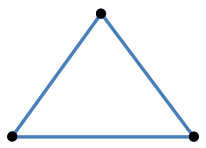
\includegraphics[width=0.3\textwidth]{./figure/triangle.png}\label{fig:triangle}}
 \subfloat[]{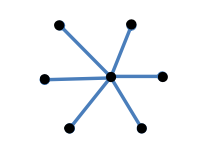
\includegraphics[width=0.3\textwidth]{./figure/spokes.png}\label{fig:spokes}}
 \subfloat[]{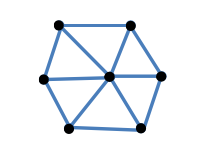
\includegraphics[width=0.3\textwidth]{./figure/spokes_and_rims.png}\label{fig:spokes_and_rims}}
 \caption{Different edge sets for triangulation mesh: (a) triangle; (b) spokes; (c) spokes-and-rims;}
 \label{fig:cell}
\end{figure}

\subsection{Linear deformation}
Linear means we use a linear system of equations to formulate a global quadratic variational minimization problem, which is the main ingredient of the deformation algorithm. The advantage of linear deformation methods are three-folds: efficient, solving a linear system of equation is quite efficient, especially when the associated linear system is sparse; robust, the solved quadratic energy has a unique global minimum; smooth, the global energy minimization guarantees smooth and $\mathcal{C}^1$ continuous surface deformations. According to the target the deformation applied onto, the linear deformation methods can be categorized into linear surface based deformation and linear space deformation.

\subsubsection{Linear surface-based deformation}
The linear surface-based deformation roughly falls into three categories: shell-based deformation, multi-scale deformation and differential coordinates based deformation.

Shell-based deformation method minimizes the elastic energy subject to user-defined boundary constraints. The elastic energy measures how much the object has been deformed from its initial configuration, which is the main requirement for physically based surface deformations. For two-manifold surfaces, the elastic energy considers local stretching and bending within the object. \cite{terzopoulos1987elastically,celniker1991deformable} propose physically-based deformation methods minimizing stretching and bending under deformation constrains, which corresponds to thin-shell models of non-planar rest states. Deformation based on a discretization of variational bending energy minimization is mathematically understood and yields smooth and tangent-continuous deformations \citep{guskov1999multiresolution,kobbelt1998interactive,botsch2004intuitive,bickel2008pose}. However, for these approaches all computations and linearizations are performed with respect to a fixed reference mesh, large deformations might lead to shape distortions and detail loss.

To preserve surface details, the above methods require a multi-scale decomposition, which splits a surface into a smooth base surface (low frequencies) and displacement vectors (high frequencies). Multiresolution deformation changes the smooth base surface and adding the details back onto it then yields the desired multi-scale deformation \citep{kobbelt1999multiresolution}. In particular, \cite{kobbelt1998interactive} introduces a mesh deformation technique by solving a constrained minimization of the thin-plate energy at a desirable coarse resolution. The user specifies deformation constraints through a handle polygon. Original mesh details are added back to the resulting smooth mesh to produce a final solution. This technique only gives the user limited control over the mesh shape through sparse constraints on the handle polygon. The rest of the mesh geometry is uniquely determined by the minimization. Displacement volumes \citep{botsch2003multiresolution} encode the high frequencies by prism elements enclosed between the original and the base surface, which avoids detail distortion, but comes at the considerably higher cost of a non-linear detail reconstruction. Although both representation (displacement vectors/volumes) can be combined with any underlying deformation technique, the required multiscale decomposition can become quite difficult for geometrically or topologically complex models.

To avoid the multi-scale decomposition, other methods modify differential surface properties instead of its spatial coordinates, and then solve a linear Poisson system for a deformed surface with the desired differential coordinates \citep{lipman2004differential,sorkine2004laplacian,yu2004mesh,zayer2005harmonic,lipman2005linear}. The methods of \cite{yu2004mesh,zayer2005harmonic} use gradients of affine deformations, i.e., their rotation and scale/shear components, for transforming surface gradients.  As a consequence, these methods work well for rotations, but are insensitive to translations: Adding a translation to a given deformation does not change its gradient, and thus has no influence on the resulting surface gradients. But since even pure translations induce local rotations of tangent planes, these methods are counter-intuitive for modifications containing large translations. In contrast, the shape editing approach of \cite{sorkine2004laplacian} aims to preserve the differential coordinates or Laplacian coordinates. It implicitly solves for local rotations of vertex neighborhoods, but due to linearizations their method has problems with large rotations, as was shown in their follow-up paper \citep{lipman2005linear}. In that paper, Lipman et al. minimize bending by preserving relative per-vertex orientations. They solve a linear system for per-vertex orientations, and reconstruct vertex positions. Since the first system does not consider position constraints, their technique also neglects the connection between translations and rotations, it exhibits the same translation-insensitivity as gradient-based methods.

\subsubsection{Linear space deformation}
The need for low-dimensional control of deformation fields was identified early in computer graphics. Among the first approaches was Free-Form Deformation \citep{sederberg1986free}, which relied on regular lattices to specify spatial deformations. It parameterizes a space deformation with a 3D lattice and provides an efficient way to apply coarse deformations to complex shapes. However, achieving a fine-scale deformation may require a detailed, hand-designed control lattice \citep{coquillart1990extended,maccracken1996free} and an large amount of user manipulation. Although more intuitive control can be provided through direct manipulation \citep{hsu1992direct}, the user is still restricted by the the expressibility of the FFD algorithm. With their Wires concept, \cite{singh1998wires} present a flexible and effective space deformation algorithm motivated by armatures used in traditional sculpting. A collection of space curves tracks deformable features of an object, providing a coarse approximation to the shape and a means to deform it. \cite{singh2000skinning} generalize this concept to a polygon-based deformer. \cite{botsch2005real} use triharmonic radial basis functions for real-time freeform shape editing. An incremental least-squares method is introduced to approximately solve the involved linear systems in a robust and efficient manner.

Cage-based deformation methods were an important step forward, because control polytopes offer much better adaptability to the input shapes. The underlying theme of many cage-based methods is to generalize barycentric coordinates from simplices to general polytopes. Mean value coordinates (MVC) for closes polyhedrons \citep{ju2005mean} offer many desirable properties and can be calculated using closed-form expressions, but are not fully shape-aware. This shortcoming has been addressed by harmonic coordinates \citep{joshi2007harmonic}. \cite{lipman2007gpu} introduce positive mean value coordinates (PMVC). Unlike the MVC, the modified coordinates are unconditionally positive, and require only a local computation. The methods mentioned above are affine-invariant and not shape-preserving. \cite{lipman2008green} introduce green coordinates for closed polyhedral cages. It does not only dependent on vertex-based basis, but also on the cage faces, which leads to space deformations with a shape-preserving property. While many new intriguing coordinates and their underlying mathematical properties have been studied in recent years \citep{hormann2008maximum,weber2011complex,li2013poisson}, the problem common to all cage-based method remains: the design of control cages requires experience with polygonal modeling: the cage should be close to the shape and have enough density to represent the shape.

\subsection{Nonlinear deformation}
The surface deformation problem is inherently non-linear, it requires deducing local rotations of the surface based on position displacements. Therefore, a linear method can only provide an approximate result, or a compromise must be made in terms of the problem setup, e.g., requiring more complex interactive input from the user, for example adding more user handle constraints or increasing the cage density. The inherent limitations of linear methods motivated us to investigate non-linear deformation techniques. Nonlinear deformation can also be classified into nonlinear surface-based deformation and nonlinear space deformation.

\subsubsection{Nonlinear surface-based deformation}
Pyramid coordinates \citep{kraevoy2004cross,kraevoy2005template} can be considered as the nonlinear versions of Laplacian coordinates, leading to differential coordinates invariant under rigid motions, which can be used for deformation as well as for morphing. \cite{huang2006subspace} employ a nonlinear version of the volumetric graph Laplacian, which also features nonlinear volume preservation constraints. In order to increase the performance and efficiency of the optimization, they use a subspace approach: the original mesh is embedded in a coarse control cage, and the optimization is performed on the cage vertices while considering the constraints from the original mesh vertices in a least-squares manner. An alternative approach to subspace methods is the handle-aware isoline technique of \citep{au2007handle}. In a preprocessing step one constructs a set of iso-lines of the geodesic distance from either the fixed regions or the handle regions. For each of these iso-lines, a local transformation for a Laplacian-based deformation is found by a nonlinear optimization. The number of required iso-lines is relatively small, which guarantees an efficient numerical optimization and thereby allows for interactive editing. \cite{shi2007mesh} combine Laplacian-based deformation with skeleton-based inverse kinematics, which allows for easy and intuitive character posing, featuring control of lengths, rigidity and joint limits, but it in turn requires a complex cascading optimization for the involved nonlinear energy minimization. \cite{botsch2006primo} propose a nonlinear version of the shell-based minimization of bending and stretching energies. The surface is modeled as a thin layer of triangular prisms, which are coupled by a nonlinear elastic energy. During deformation the prisms are kept rigid, which allows for a robust geometric optimization. A hierarchical optimization is used to increases the computational efficiency.

\cite{sorkine2007rigid} propose a surface deformation based on the as-rigid-as-possible (ARAP) energy. The ARAP energy measures the local deviation of the differential of a mapping between two shapes from rigidity. The neighboring edge sets adopted in this work are spokes, which requires a positive weighting scheme to guarantee the correct minimization of the energy. \cite{chao2010simple} take into account all the opposite edges in the triangles incident to a vertex, the neighboring edge sets in their work are spokes and rims, which guarantee correct minimization of the energy even if the weights are negative. However, the discretization of \citep{chao2010simple} is only consistent for volumetric case with tetrahedron cells in 3D or parameterization with triangle edge sets in 2D, it is not consistent for the surface case using spokes and rims edge sets in 3D. In order to come up with a consistent discretization for surface in 3D, \cite{levi2015smooth} introduce a new ARAP-type energy, named SR-ARAP (ARAP with smooth rotations), they add a bending term in the ARAP energy to enable the discretization consistent, which achieves results with quality that competes with the volume deformation.

\subsubsection{Nonlinear space deformation}
\cite{sumner2007embedded} compute detail-preserving space deformations by formulating an energy functional that explicitly penalizes deviation from local rigidity by optimizing the local deformation gradients to be rotations. In addition to static geometries, their method can also be applied to hand-crafted animations and precomputed simulations. \cite{botsch2007adaptive} extend the PriMo framework \citep{botsch2006primo} to deformations of solid objects. The input model is voxelized in an adaptive manner, and the resulting hexahedral cells are kept rigid under deformations to ensure numerical robustness. The deformation is governed by a nonlinear elastic energy coupling neighboring rigid cells. Another class of approaches uses divergence-free vector fields (the divergence of the vector fields is zero) to deform shapes \citep{angelidis2006swirling,von2006vector}. The advantage of those techniques is that by construction they yield volume-preserving and intersection-free deformations. As a drawback, it is harder to construct vector fields that exactly satisfy user-defined deformation constraints.

\cite{muller2005meshless} present meshless deformations based on shape matching. Instead of using the vertex connection information, they divide the set of vertices into clusters. Afterwards, affine transformations can be applied on each clusters. Based on this work, \cite{rivers2007fastlsm} introduce fast lattice shape matching for real-time deformation. Since the original method can be very slow for stiff models - per-vertex costs scale cubically with region width - they exploit the inherent summation redundancy of shape matching and provide large-region matching at constant per-vertex cost. With this approach, large lattices can be simulated in linear time complexity.

\cite{jacobson2013algorithms} introduces the harmonic, biharmonic, triharmoic equations w.r.t. surface displacement fields correspond to minimizers of the Dirichlet, Laplacian, Laplacian gradient energies. They offer a detail derivation to obtain a linear system to solve this second-order elliptic partial differential equation. \cite{weber2007context} uses harmonic functions that are provably monotonic and bounded but have only $C^0$ smoothness near constrained boundary. Bounded biharmonic weights are proposed in~\cite{jacobson2011bounded} to minimize the Laplacian energy subject to bound constraints. They spreads the influences of the controls in a shape-aware and localized manner, even for objects with complex and concave boundaries. \cite{jacobson2010mixed} use mixed finite elements to provide a discretization for biharmonic and triharmonic equations on meshes. They factorize the original equations into low-order equations by introducing additional variables, and introduce lumping mass matrices to eliminate unneeded variables. Their minimizers exhibit increasing orders of continuity but lose the maximum principle and show oscillations. \cite{jacobson2012smooth} propose smooth shape-aware functions with controlled extrema. They provide a framework for minimizing quadratic energies on manifolds while constraining the solution to obey the maximum principle in the solved region.

\subsection{3D geometric deformation summary}
3D geometric deformation is a crucial part of shape registration as it serves as a regularization to attract the template onto the target. This section investigates the state of the art linear and nonlinear deformation techniques, and compares them in terms of handling large deformation and consistency. The linear methods can only approximate the local rotations, which are commonly seen in surface deformation. Nonlinear approaches are able to handle local rotations. However, some of them do not allow local scales, which are required in addressing large local deformation. Although some methods allow local scale but they are not consistent, which prone to fold-over and self-intersection, especially in the case of poor triangulation. In this research, a novel deformation algorithm will be proposed to address large difference in size, as well as to guarantee the energy consistent to minimize the occurrence of fold-over and self-intersect.



\section{3D shape correspondence}
Establishing a meaningful shape correspondence is a fundamental task in applications such as object recognition, statistical shape modeling, shape morphing and deformation transfer. In this section, we will give an overview of the correspondence research from three point of views: similarity-based correspondence, rigid alignment and non-rigid alignment.

\subsection{Similarity-based correspondence} One of the most fundamental ways of computing correspondence is to estimate the similarity between pairs of shape elements or feature points collected from the shapes and derive a correspondence from those estimates, which is sometimes called the feature matching approach. The elements are commonly characterized by shape descriptors. There are plenty of shape descriptors can be computed for each shape primitive and used in conjunction with correspondence algorithms for 2D surfaces or 3D point sets (Table~\ref{tbl:descriptor}).
 
 \begin{table*}[!hptb]
%\hspace{-20in}
 
  \centering
  \begin{tabular}{  | l | l | }
     \hline
     Descriptor& Type of dataset  \\ \hline
     Shape context & Point sets\\ 
     Spin images & Oriented points\\ 
     Multi-scale features & Oriented points\\ 
     Curvature maps & Surfaces\\ 
     Integral invariants & Surfaces\\ 
     Spherical harmonics and wavelets & Surfaces\\
     Salient geometric features & Surfaces\\
     Part-aware metric & Surfaces\\
     Heat Kernel Signature & Surfaces\\ \hline
     
     
  \end{tabular}
  \caption{Shape descriptors can be used for shape correspondence.\label{tbl:descriptor}}

 \end{table*} 
 
 
 
A correspondence is obtained by selecting assignments between pairs of elements while optimizing an objective function composed of two terms. The first term seeks to maximize the similarity between the descriptors of corresponding elements, while the second term seeks to minimize the distortion that would be introduced in the shapes if they were deformed to align their corresponding elements. However, the second term can be estimated without explicitly aligning the shapes. Ideally, satisfying these objectives should translate into a solution that is geometrically or semantically meaningful. Such a solution is typically obtained with a standard optimization method (e.g., quadratic programming).

Feature matching can be applied in any context where it is possible to compute a set of descriptors for the elements. Example applications include registration of 3D scans \citep{castellani2008sparse} and deforming surfaces \citep{anguelov2005correlated}, or skeleton matching \citep{biasotti2006sub}. Moreover, this approach is not restricted to its own domain and can be combined with alignment-based approaches to provide a proper initialization to these methods \citep{rusinkiewicz2001efficient}, or to restrict the size of the solution space \citep{gelfand2005robust,kin2010electors,chang2008automatic,aiger20084}.

\subsection{Rigid alignment} Rigid alignment is to find a global geometric transformation that aligns the shapes. One example application is the rigid alignment of geometry scans used for shape acquisition. The goal here is to capture a real-world static 3D shape and obtain its digital representation. However, it may not be possible to capture the entire object in a single scanning pass due to self-occlusions and physical constraints of the scanner, so it might become necessary to acquire multiple scans and optimally align them to reconstr uct the full object \citep{turk1994zippered,rusinkiewicz2001efficient,gelfand2005robust,aiger20084}. The key characteristic of the rigid alignment problem is that the objects do not change from one scanning pass to another. Thus, it is assumed that each scan can be transformed with a single rigid transformation in order to align it perfectly with the other scans. Rigid transformations comprise mainly translations and rotations, and one of their important characteristics is that they reside in a low-dimensional space.

Scan alignment is just one example of many applications that rely on the assumption of rigidity in the datasets. If the input shapes are given as sets of 3D points, the problem of rigid alignment can be posed as: for each point set, find the rigid transformation that maximizes the number of points in the set that align to points in the other sets. This goal is usually dependent on a threshold that indicates when two points are close enough and can be considered as matching to each other \citep{irani1999combinatorial}. Since finding the best aligning transformation might be a complex task, the feature matching approach can be brought in to aid in the search for the optimal alignment.

\subsection{Non-rigid alignment} Sometimes it might be necessary to lift the assumption that each scan can be perfectly aligned with a rigid transformation, e.g., when large amounts of noise are present in the scans. More significant examples of datasets that cannot be perfectly aligned with a rigid transformation include the correspondence of articulated shapes \citep{elad2003bending,anguelov2005correlated,jain2007non,chang2008automatic,huang2008non}, where certain parts of the shapes can be bended independently, the correspondence of anatomical shapes (e.g, organs) \citep{audette2000algorithmic}, which can deform in an elastic manner and introduce stretching to localized portions of the shape, and finally the correspondence between shapes with different geometries but that represent a same class of objects or which have parts that are semantically related \citep{allen2003space,zhang2008deformation}. In the latter case, the alignment problem can be concluded as establishing a correspondence between shapes that can differ in both local stretching and bending.

To this end, it become necessary to add more degree of freedom (DOF) to how the shapes can be brought into correspondence. This can be achieved by generalizing two aspects of the problem. First, non-rigid (possibly non-linear) transformations can be taken into consideration, e.g., thin-plate splines \citep{chui2003new}. Secondly, these transformations can be applied separately to local portions of the shape. For example, the transformation applied to a shape can be represented as a set of displacement vectors ( one per shape vertex) \citep{pauly2005example}. Then, finding the best transformation amounts to computing the displacements that bring each vertex in correspondence with the target shape. The distinction to the rigid case is that the DOF of geometric transformations being considered is now inherently high-dimensional.

\subsection{3D shape correspondence summary}
In the process of shape registration, finding correspondence is the priori step before deforming the template, it determines the goal positions of the deformed template. This section reviews the methods solving rigid and non-rigid correspondence problems. Rigid alignment is only effective with static shapes. For deformable shapes, similarity-based correspondence methods work well between isometric shapes, as the descriptors it adopted can be isometrically invariant such as Heat Kernel Signature. However, there is no such shape descriptor which is invariant to large non-isometric deformation. Non-rigid alignment assumes the template can be transformed onto the target in a specified type of deformation, however, the space of solution to large deformation itself is quite high dimensional and hard to find. In this research, we design a novel matching energy to choose correspondence between non-isometric shapes, the correspondences are first chose based on local geometric feature descriptors and then extended to local optimal candidates.

\section{3D shape registration}
3D registration is an active research topic in computer graphics and computer vision. Given a template and a target, the goal of 3D registration is to find a mapping between them in order to optimally transforms the template onto the target. Shape registration methods can fall roughly into 3 classes: rigid, isometric, non-isometric.

\subsection{Rigid registration}
The purpose of rigid registration is to find a global rigid transformation that aligns two shapes. It is quite similar to rigid alignment in last subsection, just has a different final goal. The most classic algorithms for rigid registration are Iterative Close Point (ICP) \cite{besl1992method} and its variants \cite{rusinkiewicz2001efficient}. ICP alternates between searching correspondences by choosing closest points on the target w.r.t. the points on the template and computing a rigid transformation to response the correspondences. The results closely dependent on the initial position and orientation of the shapes, large distance between them tend to produce unstable correspondence and ICP is susceptible to converge to local minimum. Aiming to solve this problem, \cite{gelfand2005robust} initially approximate the optimal transformation via feature matches, this approximation can be fed into ICP to improve the converge accurate and rate. Another shortage of ICP is that it is sensitive to noise and outliers which often appear in 3D scans. To tackle this issue, \cite{bouaziz2013sparse} put forward a new variant of ICP algorithm with sparsity-inducing norms, successfully eliminating the affect of the noise and outlier and obtaining superior results.

\subsection{Isometric registration}
Isometric registration is to solve a local rigid transformation for each vertex on the template in order to align the template onto the target. \cite{li2008global} propose a isometric registration algorithm for partial scans of deforming shapes within a single non-linear optimization. The rigid energy term they adopted penalizes the deviation of each local transformation from a pure rigid motion, which is only composed of rigid and orientation transformation. \cite{qixing2008non} regard isometric registration as an optimization problem. To solve this problem, they alternate between correspondence searching and deformation calculation. Under the assumption of local rigid deformation, robust correspondence are obtained via a pruning mechanism based upon consistency in geodesic distance. \cite{chang2008automatic} convert the isometric registration problem into a discrete labeling problem. They first sample the motion explicitly, which provides a priori set of possible rigid transformation between articulate parts of shapes, then finding an optimal assignment of transformation to each part of shapes. \cite{tevs2009isometric} propose a global isometric matching approach based on a novel RANSAC-like randomized sampling algorithm. This method is robust to topological noise and is able to output matching alternatives by sampling the space of plausible solutions. \cite{maron2016point} approximate the global minimum of the procrustes matching problem with convex relaxation for non-rigid isometric and near-isometric shape matching problem. The advantage of isometric registration is that they can achieved automatically, but they are incapable of handling models with different sizes.

\subsection{Non-isometric registration}
Non-isometric registration is a wide range of topics including all kinds of registration are not isometric. Here we only focus on techniques related to our work: similar registration, affine registration and smooth registration.

\subsubsection{Similar registration}
Similar registration is to preserve the local similarity of shapes, it remains the angle of intersection of every pair of the intersecting arcs unchanged during deformation process. \cite{sorkine2004laplacian} offer a linear approximation of similarity matrix to make deformed Laplacian coordinates consistent. However, this method only works well under small rotations as the approximation removes the quadratic term. Thus it cannot handle large rotation. \cite{yamazaki2013non} extend ARAP energy to \emph{as-similar-as-possible} (ASAP) energy with spokes edge sets. The work in \citep{papazov2011deformable} is a variation of shape matching~\citep{muller2005meshless} called similarity shape matching. Although these techniques utilize similar mapping to enable them to address size difference and shear distortion, they do not consider the smoothness regularization, which results in they are incapable of handling large changes in pose or shape. \cite{yoshiyasu2014conformal} incorporate smooth regularization into the total energy, however, it is a unweighted energy, which does not take into account the impact of the length of edges. Moreover, the edge sets they adopt is spokes, which leads to an inconsistent energy.

\subsubsection{Affine registration}
Affine registration allows a affine transformation for each template vertex, which will have a larger solution space due to more freedom the affine matrix has. \cite{amberg2007optimal} employ a locally affine regularisation to each vertex and smooth the difference in the transformation of neighbouring vertices. The method is robust to incomplete data and is able to handle a wide range of initial conditions. \cite{yang2015sparse} propose a sparse non-rigid registration method with an $l_1$-norm regularized model for transformation estimation, they allow an affine transformation for each point in the template to cover a wide range of non-rigid deformations. Affine registration is able to handle shapes in different size, but the affine matrix with more DOF may also introduce shear and distortion, which easily lead to fold-over and intersection.

\subsubsection{Smooth registration}
Smooth registration is based on harmonic mapping or its varieties or other smoothness regularization. \cite{weise2009face} provide a complete integrated system for live facial puppetry which not only is able to track high-resolution facial expression in real time but also can transfer the expression to another face. They minimize a membrane energy on the displacement vectors to smooth the deformation on the template. \cite{yeh2011template} present a novel approach for template-based 3D model fitting , they approximate the input geometry with a linearized biharmonic surface, and then use iterative Laplacian editing and a local surface flattening mechanism to avoid foldovers. There are some works~\citep{allen2003space,amberg2007optimal} based on other smoothness regularization whose purpose are to make the deformation between neighbors as smooth as possible, this idea is similar to the bending term added in~\cite{levi2015smooth}. Similar to affine registration, smooth registration still has the same advantage and problem. In addition, it requires many landmarks from user input to obtain a good initial shape.

\subsection{3D shape registration Summary}
In summary, 3D shape registration with large size and detail difference is challenging problem mainly because of the requirement of large deformation which is susceptive to fold-over and intersection. This section investigate all kinds of registration methods and their capabilities. Rigid registration is only suitable for static models. Isometric registration can work with deformable objects but only limit to isometric shapes or near isometric shapes. Affine and smooth registration are able to handle models with different sizes, but they are too weak to against shear distortion. Although similar registration can overcome these disadvantages, the energy itself is not consistent, which easily leading to fold-over and self-intersection when the triangulation mesh is poor. In this research, a novel registration technique will be present to solve large shape variation as well as minimize the change of fold-over occurrence.

\ifx\isEmbedded\undefined
% References
\addcontentsline{toc}{chapter}{References}
\pagebreak
\end{document}
\fi
